\documentclass[14pt]{beamer}
%\usetheme[compress]{Singapore} % Guia no alto, nada mais, degrade azul
\usetheme{Frankfurt} % Guia no alto, nada mais
%\usepackage[latin1]{inputenc}
\usepackage[utf8]{inputenc}
\usepackage{subfigure}
\usepackage{multirow}
\usepackage{etex}
\usepackage{pstricks}
\usepackage{pstricks-add}
\usepackage{pst-plot}
\usepackage{pst-xkey}
\usepackage{pst-3dplot}
\usepackage{pst-node}
\usepackage{pst-all}
\usepackage{./pst-exa}
\usepackage{tikz}
% \usepackage[english]{babel}    % se o documento for em inglês
%\usepackage[latin1]{inputenc}
% \usepackage[latin1]{inputenc}
\usepackage{fontenc}
\usepackage{type1ec}
\usepackage{graphicx}
\usepackage{float}
\setbeamertemplate{navigation symbols}{}

\title{Economically-Efficient\\Data Stream Analysis}
\author{\small{Roberto Oliveira Jr.\\Orietador: Adriano Veloso \\Co-orientados: Wagner Meira Jr.}}
\institute{DCC - UFMG - Brazil}
\date{}

\begin{document}

\begin{frame}
\titlepage
\end{frame}

\section{Análise de Fluxos de Dados}

\begin{frame}\frametitle{Fluxo de Dados}

\begin{itemize}
\item Definição
\begin{itemize}
\item Sequência de dados possivelmente ilimitada, de alta velocidade onde os dados chegam em intervalos de tempos variados.
\end{itemize}
\item Motivação
\begin{itemize}
\item Permite o processamento de grandes volumes de dados.
\end{itemize}
\end{itemize}
\begin{itemize}
\item Problema
\begin{itemize}
\item Extrair automaticamente padrões e relações relevantes de dados continuamente criados.
% \begin{itemize}
% \item Keep track of data streams is useful for systems monitoring, online social network advertising, etc.
% \end{itemize}
\end{itemize}
\end{itemize}

\end{frame}

% \begin{frame}\frametitle{Social Networks Streams and Advertising}

% {\underline{FIFA World Cup 2014}}

% \begin{figure}
% \centering
% 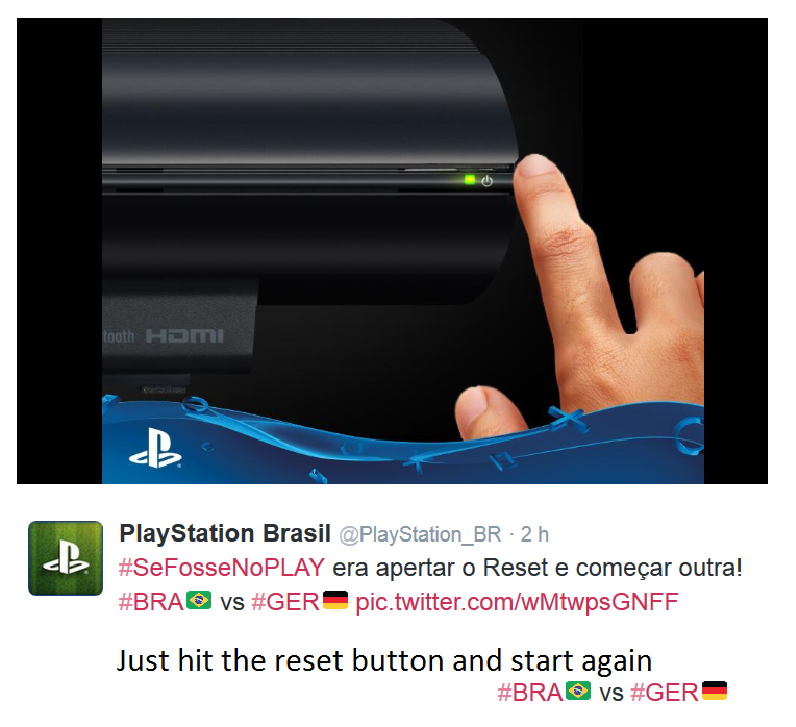
\includegraphics[scale=0.65]{playstation}
% \end{figure}

% \end{frame}

\begin{frame}\frametitle{Classificação em Fluxo de Dados}

\begin{itemize}
\item Modelos de classificação são aplicados para distinguir entre rótulos pré-estabelecidos.
\end{itemize}

\vspace{-0.2in}
\begin{figure}
\centering
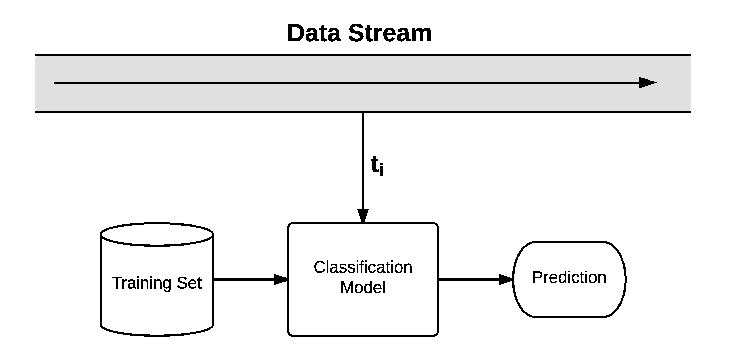
\includegraphics[scale=0.6]{Stream1}
\end{figure}
\vspace{-0.2in}
\begin{itemize}
\item \alert{As características dos dados podem mudar ao longo do tempo}.
\end{itemize}
\end{frame}

\begin{frame}\frametitle{Mudanças de Conceito}
\begin{itemize}
\item Mudança de Conceito é a alteração imprevisível da natureza dos dados ao longo do tempo.
\end{itemize}

\vspace{-0.5in}

\def\tiny{\fontsize{9pt}{12pt}\selectfont}
\begin{figure}[!h]
\centering
\psscalebox{1 1}{
\begin{pspicture}(-2.7,-0.5)(8.1,2.5)
%Axis

%Sudden
\rput(-2.7,0.4){\psaxes[linecolor=black,
axesstyle=axes, labels=none, ticks=none]{->}(0,0)(0,0)(2.5,2)}

\psdots[linecolor=black, dotsize=0.2](-2.5,0.6)
\psdots[linecolor=black, dotsize=0.2](-2.3,0.6)
\psdots[linecolor=black, dotsize=0.2](-2.1,0.6)
\psdots[linecolor=black, dotsize=0.2](-1.9,0.6)
\psdots[linecolor=black, dotsize=0.2](-1.7,0.6)

\psline(-1.7,0.6)(-1.3,2)

\psdots[linecolor=black, dotsize=0.2](-1.3,2)
\psdots[linecolor=black, dotsize=0.2](-1.1,2)
\psdots[linecolor=black, dotsize=0.2](-0.9,2)
\psdots[linecolor=black, dotsize=0.2](-0.7,2)
\psdots[linecolor=black, dotsize=0.2](-0.5,2)

\rput[bl](-2.5,-0.25){\tiny sudden/abrupt}

%Incremental
\rput(0.1,0.4){\psaxes[linecolor=black,
axesstyle=axes, labels=none, ticks=none]{->}(0,0)(0,0)(2.5,2)}

\psdots[linecolor=black, dotsize=0.2](0.3,0.6)
\psdots[linecolor=black, dotsize=0.2](0.5,0.6)
\psdots[linecolor=black, dotsize=0.2](0.7,0.6)
\psdots[linecolor=black, dotsize=0.2](0.9,0.6)
\psdots[linecolor=black, dotsize=0.2](1.1,0.6)

\psline(1.1,0.6)(1.9,2)

\psdots[linecolor=black, dotsize=0.2](1.25,0.8)
\psdots[linecolor=black, dotsize=0.2](1.34,1)
\psdots[linecolor=black, dotsize=0.2](1.43,1.2)
\psdots[linecolor=black, dotsize=0.2](1.55,1.4)
\psdots[linecolor=black, dotsize=0.2](1.67,1.6)
\psdots[linecolor=black, dotsize=0.2](1.77,1.8)
\psdots[linecolor=black, dotsize=0.2](1.87,2)

\psdots[linecolor=black, dotsize=0.2](1.9,2)
\psdots[linecolor=black, dotsize=0.2](2.1,2)
\psdots[linecolor=black, dotsize=0.2](2.3,2)
\psdots[linecolor=black, dotsize=0.2](2.5,2)

\rput[bl](0.6,-0.2){\tiny incremental}

%Gradual
\rput(2.9,0.4){\psaxes[linecolor=black,
axesstyle=axes, labels=none, ticks=none]{->}(0,0)(0,0)(2.5,2)}
\psdots[linecolor=black, dotsize=0.2](3.1,0.6)
\psdots[linecolor=black, dotsize=0.2](3.3,0.6)
\psdots[linecolor=black, dotsize=0.2](3.5,0.6)
\psline(3.5,0.6)(3.7,2)
\psdots[linecolor=black, dotsize=0.2](3.7,2)
\psline(3.7,2)(3.9,0.6)

\psdots[linecolor=black, dotsize=0.2](3.9,0.6)

\psline(3.9,0.6)(4.1,2)
\psdots[linecolor=black, dotsize=0.2](4.1,2)
\psdots[linecolor=black, dotsize=0.2](4.3,2)
\psline(4.3,2)(4.5,0.6)

\psdots[linecolor=black, dotsize=0.2](4.5,0.6)
\psline(4.5,0.6)(4.7,2)

\psdots[linecolor=black, dotsize=0.2](4.7,2)
\psdots[linecolor=black, dotsize=0.2](4.9,2)
\psdots[linecolor=black, dotsize=0.2](5.1,2)

\rput[bl](3.5,-0.25){\tiny gradual}

%Recurrent
\rput(5.7,0.4){\psaxes[linecolor=black,
axesstyle=axes, labels=none, ticks=none]{->}(0,0)(0,0)(2.5,2)}
\psdots[linecolor=black, dotsize=0.2](5.9,0.6)
\psdots[linecolor=black, dotsize=0.2](6.1,0.6)
\psdots[linecolor=black, dotsize=0.2](6.3,0.6)
\psdots[linecolor=black, dotsize=0.2](6.5,0.6)

\psline(6.5,0.6)(6.7,2)

\psdots[linecolor=black, dotsize=0.2](6.7,2)
\psdots[linecolor=black, dotsize=0.2](6.9,2)
\psdots[linecolor=black, dotsize=0.2](7.1,2)
\psdots[linecolor=black, dotsize=0.2](7.3,2)

\psline(7.3,2)(7.5,0.6)

\psdots[linecolor=black, dotsize=0.2](7.5,0.6)
\psdots[linecolor=black, dotsize=0.2](7.7,0.6)
\psdots[linecolor=black, dotsize=0.2](7.9,0.6)
\psdots[linecolor=black, dotsize=0.2](8.1,0.6)

\rput[bl](6.4,-0.25){\tiny recurrent}
\end{pspicture}
}
%\caption{Patterns of changes over time.}
\label{fig:cd}
\end{figure}
\vspace{-0.5in}
% \begin{figure}
% \centering
% 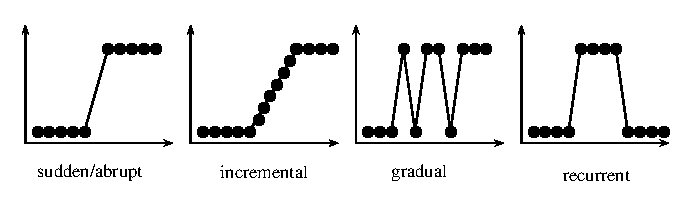
\includegraphics[scale=1]{concept_drift}
% \end{figure}
\pause

\begin{itemize}
\item Fluxo de dados contém combinação destes padrões.
\end{itemize}
\end{frame}


% \begin{frame}\frametitle{Sports (WC 2010)}

% \vspace{-0.1in}
% \begin{figure}
% \centering
% 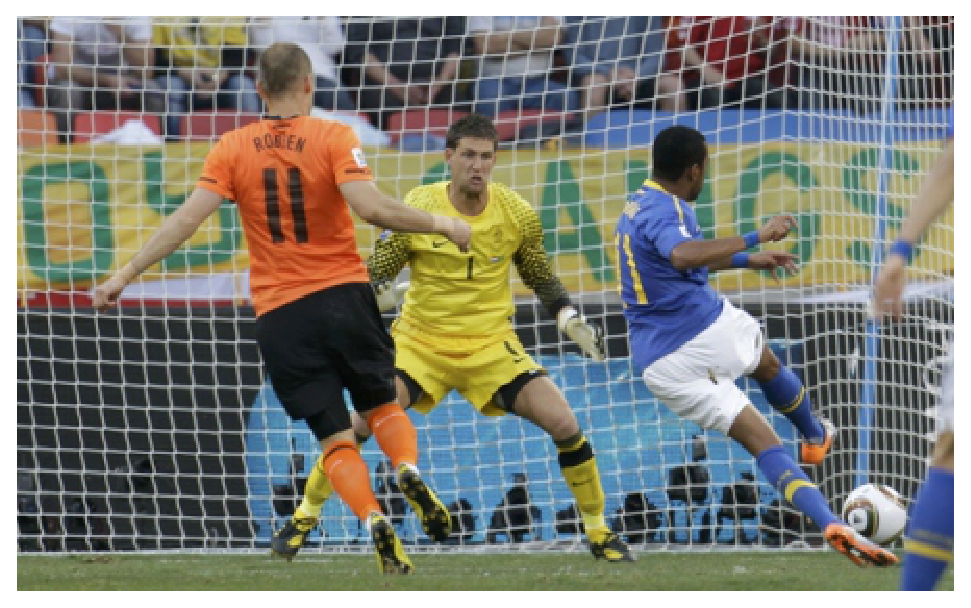
\includegraphics[height=1.00in]{golrobinho.eps}
% 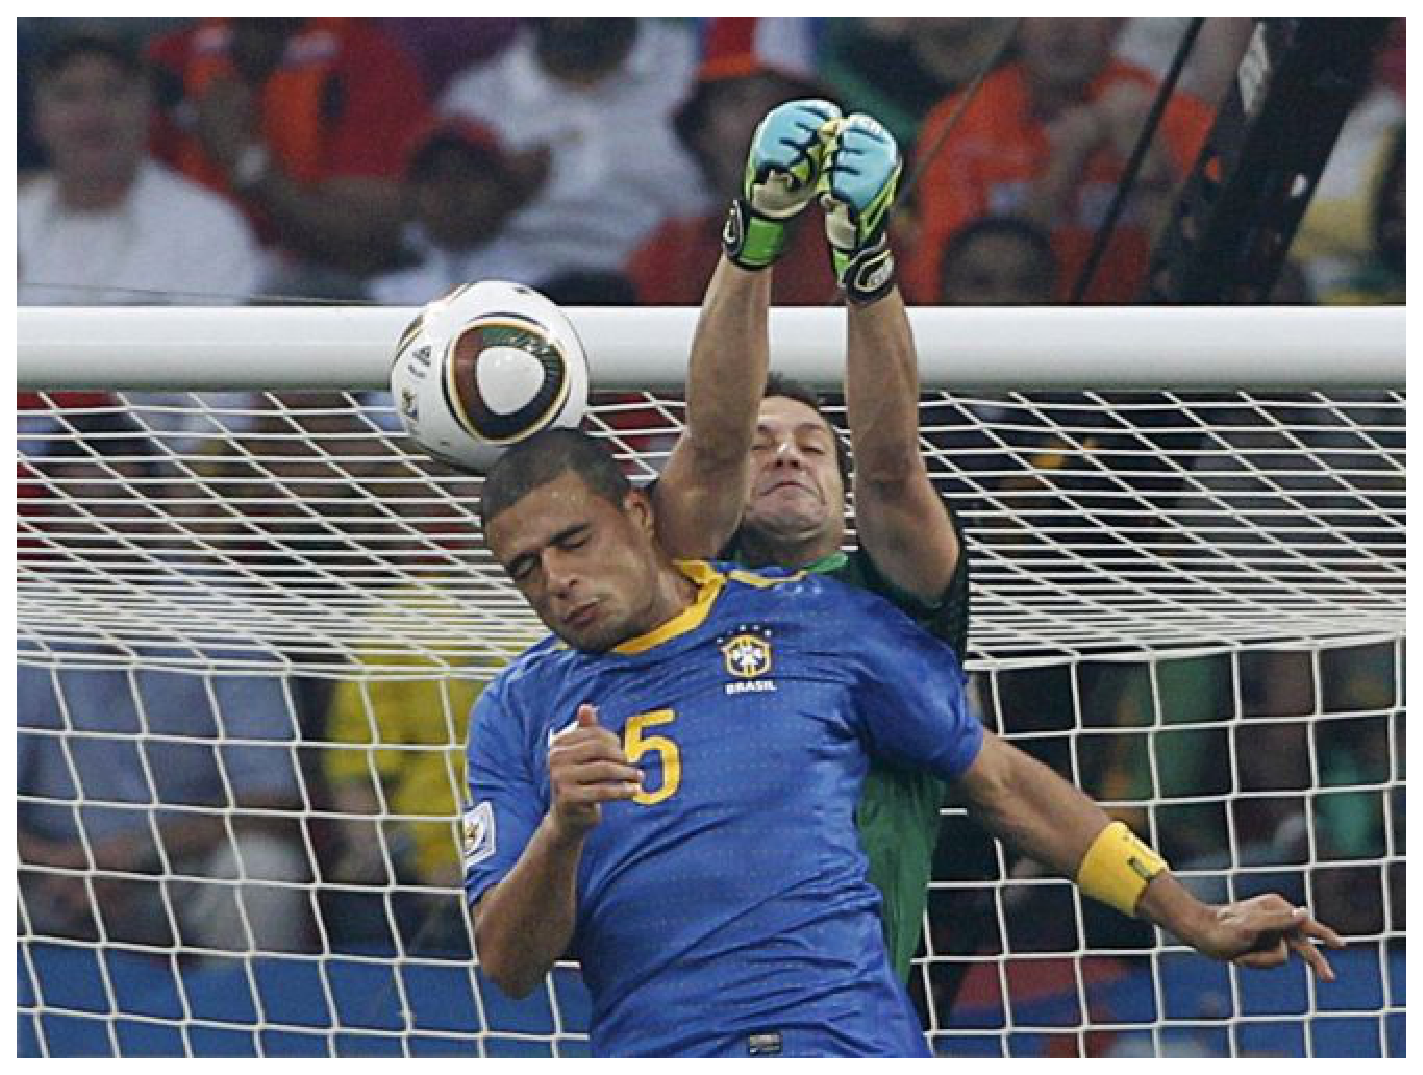
\includegraphics[height=1.00in]{contra.eps}
% 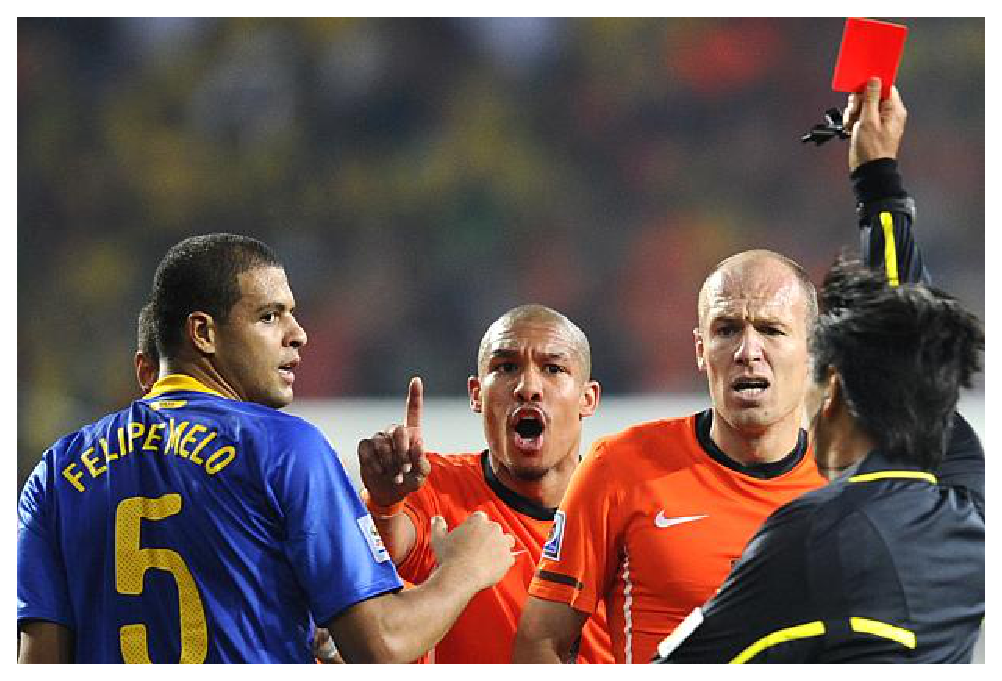
\includegraphics[height=1.00in]{vermelho.eps}
% \end{figure}

% \vspace{-0.15in}
% \begin{figure}
% \centering
% 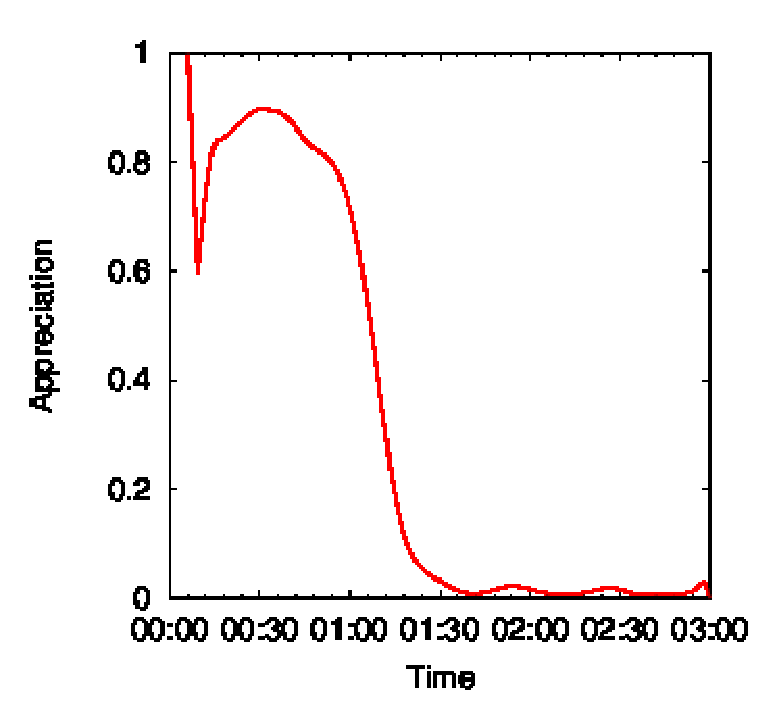
\includegraphics[width=2.35in,height=1.75in]{felipemeloPositividade.eps}
% \end{figure}

% \end{frame}

% \begin{frame}\frametitle{Elections (Brazil 2010)}

% \vspace{-0.1in}
% \begin{figure}
% \centering
% \includegraphics[height=0.95in]{dilma1}
% \includegraphics[height=0.95in]{lula}
% \includegraphics[height=0.95in]{copa}
% \end{figure}

% \vspace{-0.15in}
% \begin{figure}
% \centering
% 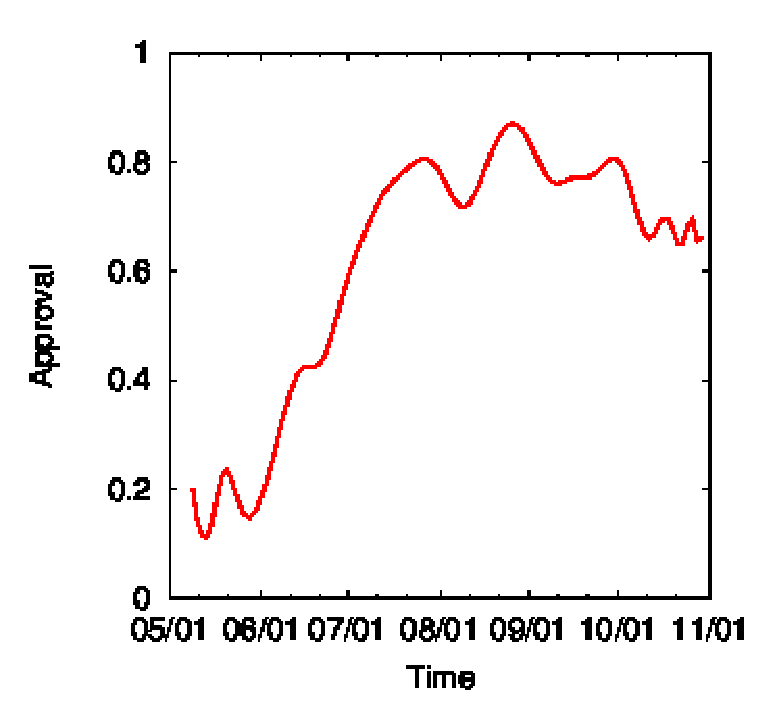
\includegraphics[width=2.35in,height=1.75in]{dilmaPositividade.eps}
% \end{figure}

% \end{frame}

\begin{frame}\frametitle{Classificação em Fluxo de Dados}

\begin{itemize}
\item Classificação efetiva requer::
\begin{itemize}
\item Atualização do modelo de classificação à medida que o fluxo evolui.
\begin{itemize}
\item Considerar limitação de recursos: memória, tempo and dados rotulados.
\end{itemize}
\end{itemize}
\end{itemize}

\vspace{-0.2in}
\begin{figure}
\centering
\includegraphics[height=1.60in]{Stream2}
\end{figure}
\end{frame}


\begin{frame}\frametitle{Questão de Pesquisa}

\begin{center}
\large{Como lidar com mudanças de conceito?}
\end{center}
% \vspace{0.5in}
% \small{\begin{enumerate}
% \item Which classification model choose?
% \item How to reduce labeling efforts?
% \end{enumerate}}
\end{frame}

\section{Economically-Efficient Selective Sampling}
%\section{Classification Model}
\begin{frame}\frametitle{Modelo de Classificação}
\begin{itemize}
\item Modelos de classificação compostos por regras de associação.
  \begin{itemize}
    \item $\{x \to y\}$, onde $x \in X$ e $y \in Y$
  \end{itemize}
\item Atualização eficiente à medida que o conjunto de treino evolui.
\item Modelos são construidos sob demanda:
  \begin{itemize}
    \item Para um dado $[x_i, *]$, regras $\{x \to y\}$ tal que $x \subseteq x_i$ são produzidas.
    \item Previsão é realizada pela combinação destas regras.
  \end{itemize}
\item A cada instante é produzido um modelo $\mathcal{R}(x_i)$.
\end{itemize}
\end{frame}

%\section{Drifts}
\begin{frame}\frametitle{Lidando com Mudanças de Conceito}

\begin{itemize}
\item Duas propriedades são necessárias para produzir modelos de classificação robustos a mudanças nos dados:
\begin{itemize}
\item Adaptação:
\begin{itemize}
\item Abilidade de adaptar às mudanças.
\end{itemize}
\item Memorização:
\begin{itemize}
\item Capacidade de recuperar após mudanças.
\end{itemize}
\end{itemize}
\end{itemize}

\begin{figure}
\centering
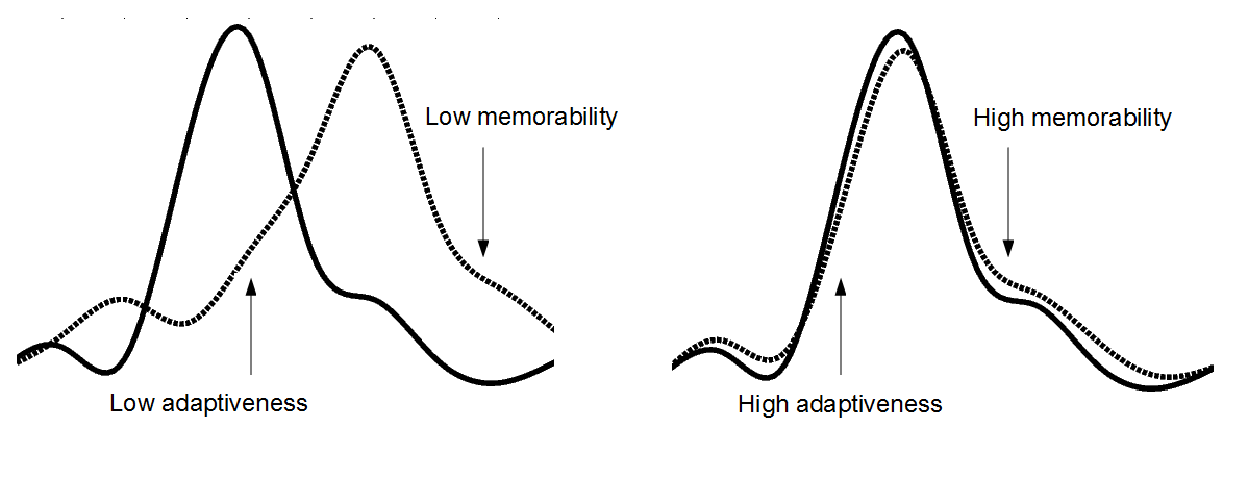
\includegraphics[height=1.30in]{drift3}
\end{figure}
\end{frame}

\begin{frame}\frametitle{Dealing with Drifts}

\begin{itemize}
\item Otimizando ambas propriedades leva a um problema de conflito de objetivo.
\begin{itemize}
\item Otimizar adaptação pode prejudicar memorização, e vice-versa.
\end{itemize}
\end{itemize}

\end{frame}


\begin{frame}\frametitle{Eficiência Econômica}

Exemplo: Hotéis em Petr\'{o}polis.

\centering

\begin{figure}[t!]
\centering
\psscalebox{0.8 0.8}{
\begin{pspicture}(0,0)(6.5,5)
   \psaxes[labels=none,ticks=none,linewidth=0.5pt,arrowscale=1.5]{->}(0.5,0.3)(0.5,0.3)(5.4,4.5)
   \rput{90}(0.15, 2.5){Memorability}
   \rput[c](3.2,0){Adaptiveness}

   \rput[c](1,4){$\circ$}
   %\psline{-}(2,4)(3.3,3.5)
   \rput[c](2.3,3.5){$\circ$}
   %\psline{-}(3.3,3.5)(4.2,3)
   \rput[c](3.2,3){$\circ$}
   %\psline{-}(4.2,3)(5.6,1.7)
   \rput[c](4.6,1.7){$\circ$}
   %\psline{-}(5.6,1.7)(6.1,0.5)
   \rput[c](5.1,0.5){$\circ$}

   %\psline{-}(1.9,3.5)(6.1,0.5)

   \rput[c](1.5,3.5){$\circ$}
   \rput[c](1.8,3.2){$\circ$}
   \rput[c](2.8,2.9){$\circ$}
   \rput[c](3.1,2.6){$\circ$}
   \rput[c](4.0,1.7){$\circ$}
   \rput[c](4.4,1.2){$\circ$}
   \rput[c](1.2,1.7){$\circ$}
   \rput[c](0.9,3.1){$\circ$}
   \rput[c](1.3,2.5){$\circ$}
   \rput[c](1.8,2.5){$\circ$}
   \rput[c](3.2,1.1){$\circ$}
   \rput[c](2.0,0.6){$\circ$}
   \rput[c](1.8,2.5){$\circ$}
   \rput[c](3.1,0.7){$\circ$}
   \rput[c](4.1,0.8){$\circ$}
   \rput[c](2.1,1.7){$\circ$}

\end{pspicture}
}
\end{figure}

% \begin{figure}
% \centering
% \includegraphics[height=1.60in]{hotel1}
% \end{figure}

\end{frame}

\begin{frame}\frametitle{Eficência de Pareto}

Fronteira de Pareto - Pontos Dominantes

\begin{itemize}
\item $U_c(a)\ge U_c(b)$ e $U_d(a)\ge U_d(b)$
\item $U_c(a) > U_c(b)$ ou $U_d(a) > U_d(b)$
\end{itemize}

\include{tt_pareto}
% \begin{figure}
% \centering
% \includegraphics[height=1.60in]{hotel2}
% \end{figure}

\end{frame}

\begin{frame}\frametitle{Compensação $-$ Princípio de Kaldor-Hicks}

Região de Compensação:

\begin{itemize}
\item Utilidade total: $U(d_i)=U_m(d_i)+U_a(d_i)$
\item Ponto base: $d^*=\{d_i\in\mathcal{P}_n | \forall d_j\in\mathcal{P}_n: U(d_i)\leq U(d_j)\}$
\end{itemize}

\begin{figure}[t!]
\centering
\psscalebox{0.8 0.8}{
\begin{pspicture}(0,0)(6.5,5)
   \psaxes[labels=none,ticks=none,linewidth=0.5pt,arrowscale=1.5]{->}(0.5,0.3)(0.5,0.3)(5.4,4.5)
   \rput{90}(0.15, 2.5){Memorability}
   \rput[c](3.2,0){Adaptiveness}

   \rput[c](1,4){$\bullet$}
   \psline{-}(1,4)(2.3,3.5)
   \rput[c](2.3,3.5){$\bullet$}
   \psline{-}(2.3,3.5)(3.2,3)
   \rput[c](3.2,3){$\bullet$}
   \psline{-}(3.2,3)(4.6,1.7)
   \rput[c](4.6,1.7){$\bullet$}
   \psline{-}(4.6,1.7)(5.1,0.5)
   \rput[c](5.1,0.5){$\color{red}\bullet$}

   \psline{-}(0.5,4)(5.0,0.3)

   \rput[c](1.5,3.5){$\bullet$}
   \rput[c](1.8,3.2){$\bullet$}
   \rput[c](2.8,2.9){$\bullet$}
   \rput[c](3.1,2.6){$\bullet$}
   \rput[c](4.0,1.7){$\bullet$}
   \rput[c](4.4,1.2){$\bullet$}
   \rput[c](1.2,1.7){$\circ$}
   \rput[c](0.9,3.1){$\circ$}
   \rput[c](1.3,2.5){$\circ$}
   \rput[c](1.8,2.5){$\circ$}
   \rput[c](3.2,1.1){$\circ$}
   \rput[c](2.0,0.6){$\circ$}
   \rput[c](1.8,2.5){$\circ$}
   \rput[c](3.1,0.7){$\circ$}
   \rput[c](4.1,0.8){$\circ$}
   \rput[c](2.1,1.7){$\circ$}

\end{pspicture}
}
\end{figure}

% \begin{figure}
% \centering
% \includegraphics[height=1.60in]{hotel3}
% \end{figure}

\end{frame}

\begin{frame}\frametitle{Medidas de Utilidade}
\begin{itemize}
\item Distância no espaço:
\begin{itemize}
\item Similariade de cada instância de treino $t_j$ em relação a nova instância $t_n$.
\item $U_s(t_j)=\frac{|\mathcal{R}(t_n) \cap \mathcal{R}(t_j)|}{|\mathcal{R}(t_n)|}$
\end{itemize}
\item Distância no tempo:
\begin{itemize}
\item Tempo de chegada de cada instância de treino $t_j$.
\item $U_t(t_j)=\frac{\gamma(t_j)}{\gamma(t_n)}$.
\begin{itemize}
\item $\gamma(t_j)$ retorna o tempo em que a instância de treino $t_j$ foi processada.
\end{itemize}
\end{itemize}
\item Permutação aleatória das instâncias de treino:
\begin{itemize}
\item $U_r(t_j)=\frac{\alpha(t_j)}{|\mathcal{D}_n|}$
\begin{itemize}
\item $\alpha(t_j)$ retorna a posição de $t_j$ na permutação.
\item $\mathcal{D}_n$ é o conjunto de treino a cada momento $n$.
\end{itemize}
\end{itemize}
\end{itemize}

\end{frame}

\begin{frame}\frametitle{Espaço de Utilidade}

\begin{enumerate}
\item Coloque as instâncias de treino no espaço de utilidade.
\item Selecione as instâncias na Região de Eficiência:
\begin{itemize}
\item Pareto-Efficience Selective Sampling (PESS)
\item Kaldor-Hicks Selective Sampling (KHSS).
\end{itemize}
\end{enumerate}

\vspace{-0.1in}
\begin{figure}
\centering
\includegraphics[scale=0.37]{pareto}
\end{figure}

\end{frame}

%\section{Labeling Efforts}
\begin{frame}\frametitle{Redução do Esforço de Rotuação}
\begin{itemize}
\item Amostragem Ativa Aleatória
\begin{itemize}
\item Estratégia ingênua.
\item Simples para integrar.
\item Controle de Esforço de Rotulação: $\beta$.
\end{itemize}
\end{itemize}
\end{frame}

%\section{EESS}
\begin{frame}\frametitle{Economically-Efficient Selective Sampling}
\begin{figure}
\centering
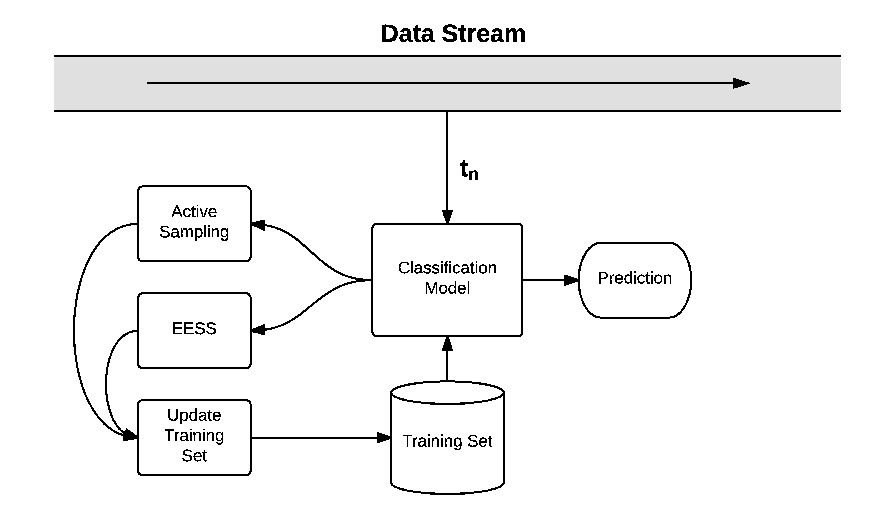
\includegraphics[scale=0.7]{EESS}
\end{figure}
\end{frame}

\section{Resultados}
\begin{frame}
\frametitle{Avaliação}
\framesubtitle{Setup}
\begin{itemize}
    \item Interleaved Test-Then-Train.
    \item 1\% do conjunto de dados provido como conjunto de treino.
    \item Ambiente de avaliação: Massive Online Analysis (MOA) framework.
    \item Baselines:
\begin{table}
\centering
\scalebox{0.6}{
\begin{tabular}{lll}
\hline
Algoritmo & Adaptação & Memorização \\
\hline \hline
AC (KDD 2011) & Aprendizado Ativo & Classificador base \\
HAT (JMLR 2011) & ADWIN & Conjunto de Árvores \\
ILAC (SIGIR 2011) & Projeção de dados & Conjunto de treino incremental\\
\hline
% EESS (SIGIR 2014) & Active Learning \& EESS & EESS \\
% \hline
\end{tabular}
}
\end{table}
\end{itemize}


\end{frame}

\begin{frame}\frametitle{Avaliação}

\begin{itemize}
\item Métricas:
\begin{itemize}
\item Erro Quadrático Médio.
\item Esforço de Rotuação: 10\%; \textbf{25\%}; 50\%; 75\% and 100\%;
\begin{itemize}
\item AC e EESS.
\end{itemize}
\item Tamanho do conjunto de treino.
\item RAM-Hours.
\end{itemize}
\item Conjuntos de Dados:
\end{itemize}
\begin{table}
\centering
\scalebox{0.6}{
\begin{tabular}{lcccc}
\hline
& \multicolumn{4}{c}{Padrão de Mudança de Conceito} \\ \cline{2-5}
 & Repentino & Incremental & Gradual & Recorrente \\
\hline \hline
Eleições Presidenciais 2010 & - & X & X & - \\
Pessoa do Ano 2015 & - & X & X &  - \\
\textbf{Copa do Mundo 2010 - Inglês} & X & - & - & - \\
\textbf{Copa do Mundo 2010 - PT} & X & - & - & -  \\
\textbf{Tipo de Cobertura} & X & - & X & X \\
Filtragem de Spam & X & - & X & X \\
\textbf{Mão de Poker} & - & - & X & X \\
\hline
\end{tabular}
}
\end{table}
\end{frame}

% \begin{frame}\frametitle{Datasets}
% \begin{itemize}
% \item Seven datasets from different applications:
% \begin{itemize}
% \item Sentiment Analysis
% \item Forest cover type prediction
% \item Spam filtering
% \item Poker game
% \end{itemize}
% \end{itemize}

% \end{frame}

% \begin{frame}
% \frametitle{Evaluation}
% \framesubtitle{Brazilian Presidential Elections}
% MSE and Labeling Efforts
% \begin{figure}[htp!]
% \label{fig:dilma_1}
% \centering
% 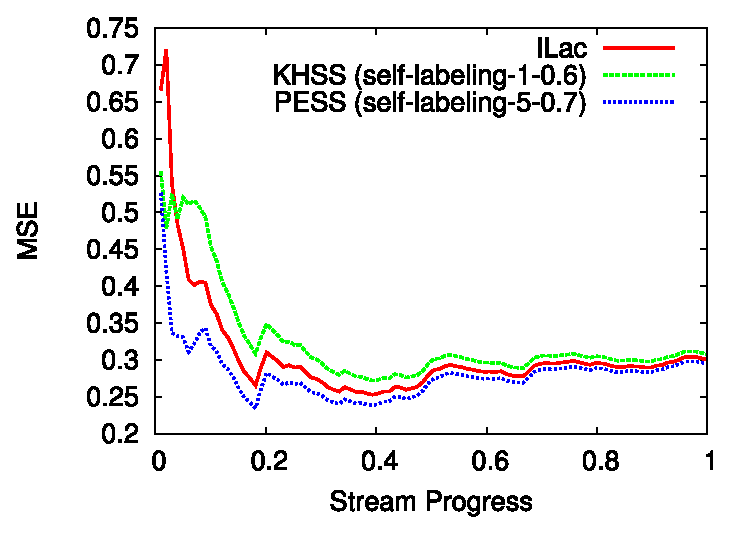
\includegraphics[scale=0.41]{dilma_mse.eps}
% \includegraphics[scale=0.41]{dilma_le_mse.eps}
% \end{figure}
% \end{frame}

% \begin{frame}
% \frametitle{Evaluation}
% \framesubtitle{Brazilian Presidential Elections}
% Training Size and RAM-Hours
% \begin{figure}[htp!]
% \label{fig:dilma_2}
% \centering
% 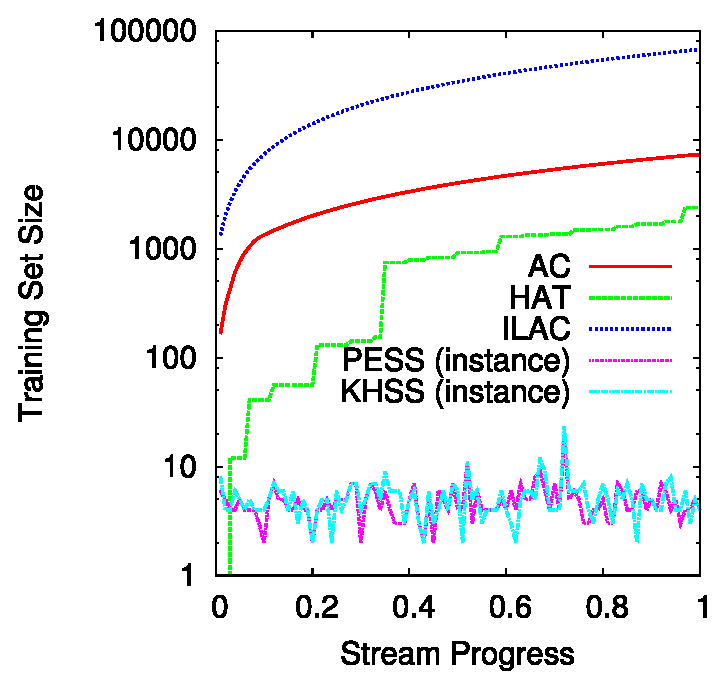
\includegraphics[scale=0.41]{dilma_window.eps}
% \includegraphics[scale=0.41]{dilma_ramhours.eps}
% \end{figure}
% \end{frame}

% \begin{frame}\frametitle{Evaluation}
% \framesubtitle{FIFA World Cup - Portuguese}
% \vspace{-0.1in}
% \begin{figure}
% \centering
% 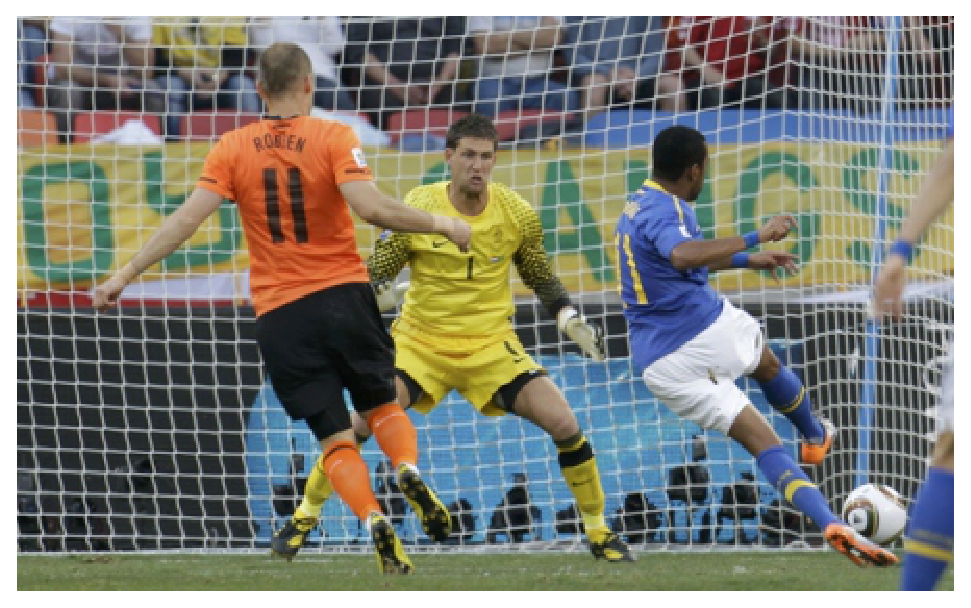
\includegraphics[height=0.9in]{golrobinho.eps}
% 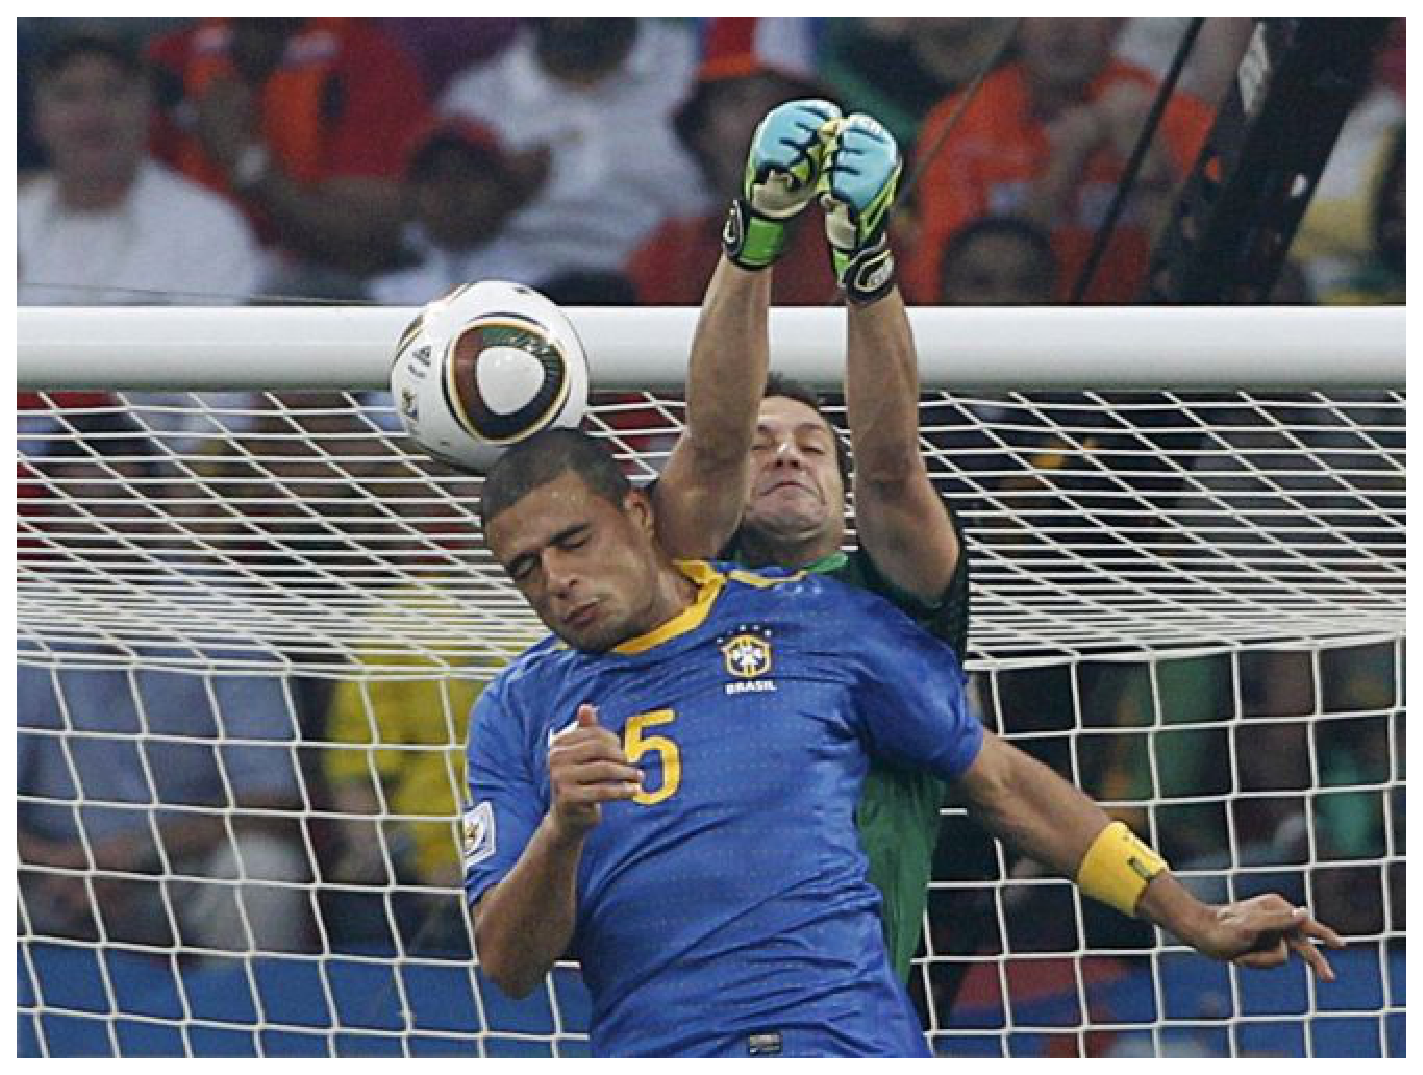
\includegraphics[height=0.90in]{contra.eps}
% 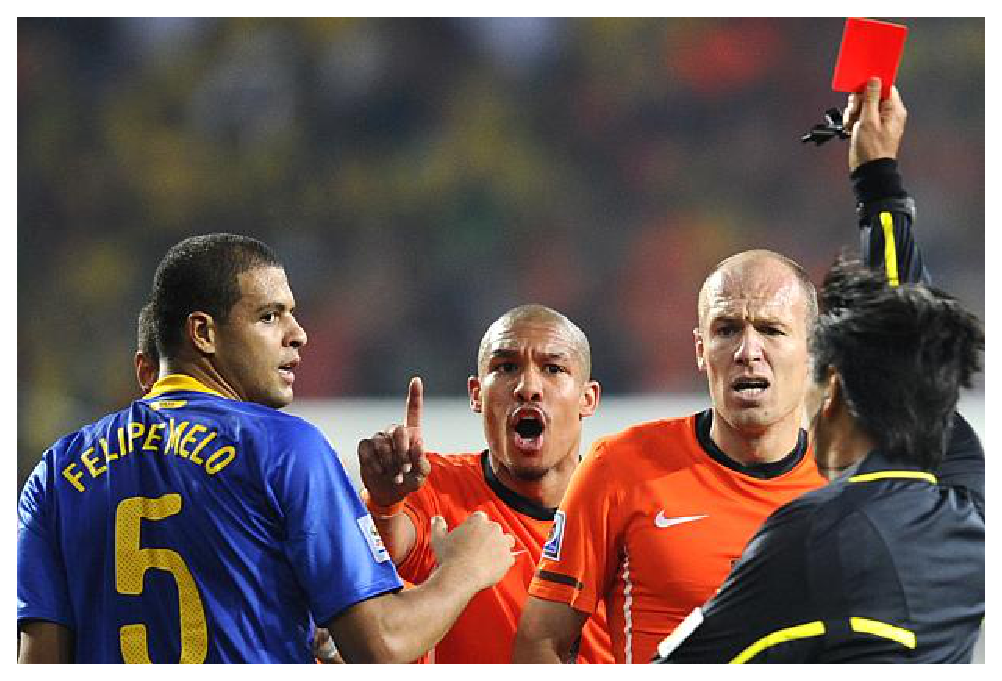
\includegraphics[height=0.90in]{vermelho.eps}
% \end{figure}

% \vspace{-0.15in}
% \begin{figure}
% \centering
% 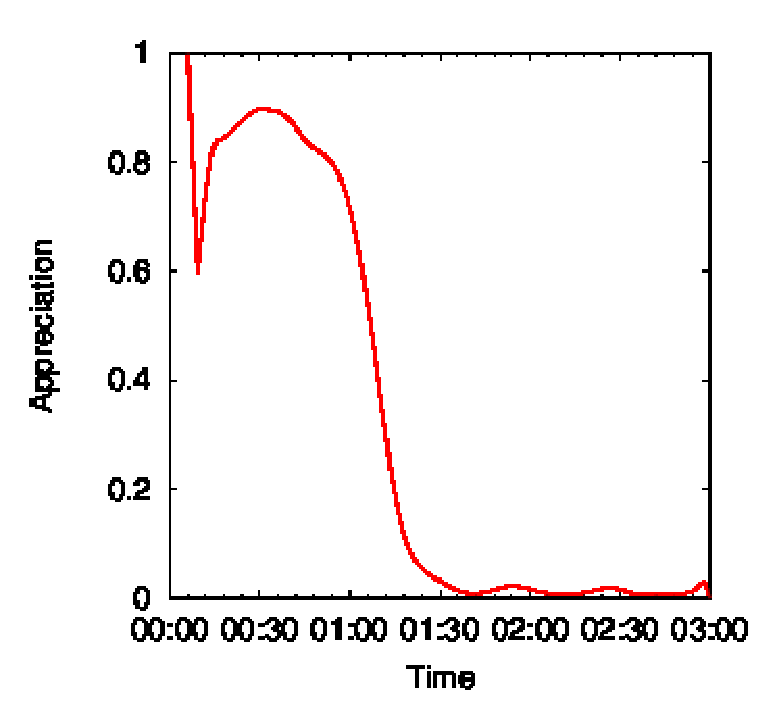
\includegraphics[scale=0.41]{felipemeloPositividade.eps}
% \end{figure}

% \end{frame}

% \begin{frame}
% \frametitle{Evaluation}
% \framesubtitle{FIFA World Cup - Portuguese}
% %MSE and Labeling Efforts
% \begin{figure}[htp!]
% \label{fig:fm_1}
% \centering
% %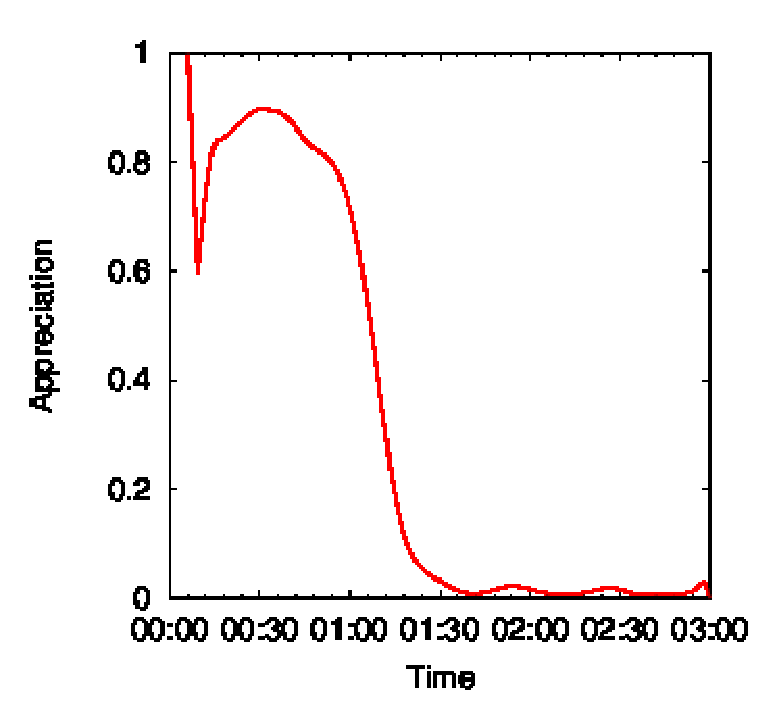
\includegraphics[scale=0.41]{felipemeloPositividade.eps}
% 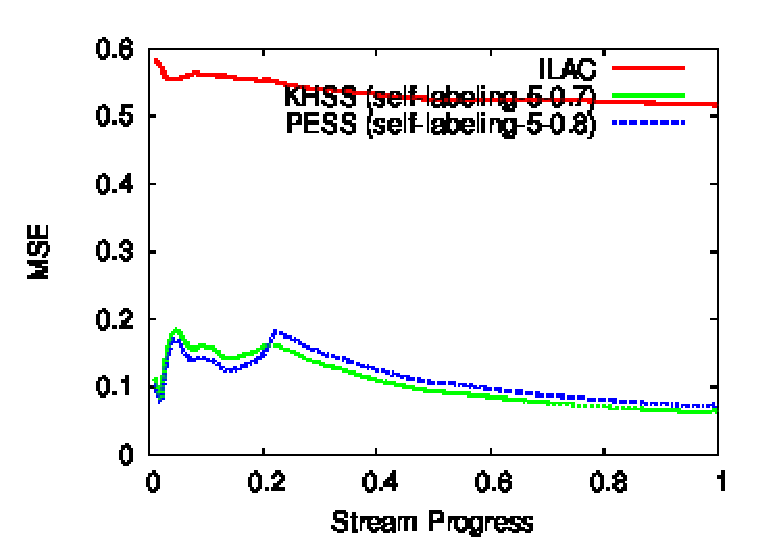
\includegraphics[scale=0.45]{pt_mse.eps}
% \includegraphics[scale=0.45]{pt_le_mse.eps}
% \end{figure}
% \end{frame}

% \begin{frame}
% \frametitle{Evaluation}
% \framesubtitle{FIFA World Cup - Portuguese}
% Training Size and RAM-Hours
% \begin{figure}[htp!]
% \label{fig:fm_2}
% \centering
% \includegraphics[scale=0.45]{pt_window.eps}
% 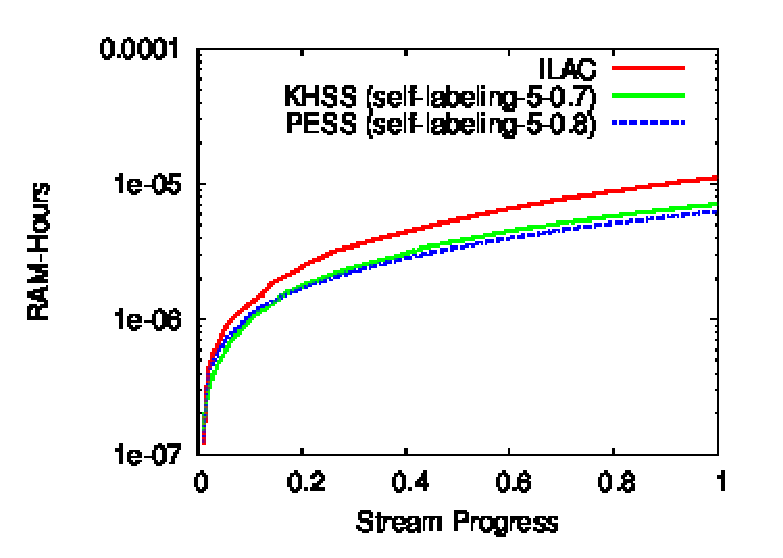
\includegraphics[scale=0.45]{pt_ramhours.eps}
% \end{figure}
% \end{frame}

\begin{frame}
\frametitle{Evaluation}
\framesubtitle{Tipo de cobertura de florestas}
\begin{itemize}
    \item Tipo de cobertura de florestas nos EUA.
    \item 581,102 instâncias com 54 variáveis e 7 classes;
    \item Mudanças de Conceito: Repentina, Gradual, Recorrent;
\end{itemize}
\begin{figure}[htp!]
\centering
\includegraphics[scale=0.3]{covtype_class_stream_1.eps}
\includegraphics[scale=0.3]{covtype_class_stream_2.eps}
\includegraphics[scale=0.3]{covtype_class_stream_3.eps}
\end{figure}

\end{frame}

\begin{frame}
\frametitle{Evaluation}
\framesubtitle{Tipo de cobertura de florestas}
MSE and Esforço de Rotulação:
\begin{figure}[htp!]
\centering
\includegraphics[scale=0.41]{covtype_mse.eps}
\includegraphics[scale=0.41]{covtype_le_mse.eps}
\end{figure}
\end{frame}

\begin{frame}
\frametitle{Evaluation}
\framesubtitle{Tipo de cobertura de florestas}
Tamanho do conjunto de treino e RAM-Hours
\begin{figure}[htp!]
\centering
\includegraphics[scale=0.41]{covtype_window.eps}
\includegraphics[scale=0.41]{covtype_ramhours.eps}
\end{figure}

\end{frame}

\section{Conclusões}

\begin{frame}\frametitle{Conclusões}
\begin{itemize}
\item Análise de Fluxos de Dados.
\begin{itemize}
\item Limitação de recursos.
\item Mudanas de Conceito.
\end{itemize}
\pause
\item Eficência e Precisão.
\begin{itemize}
\item Modelo de classificação incremental.
\item Adaptação e Memorização.
\item Eficência de Pareto e princípio de compensação.
\item Medidas de utilidade simple de computar.
\item Nossos algoritmos se mostraram robustos em diferentes cenários.
\end{itemize}
\pause
\item Trabalho futuros:
\begin{itemize}
\item Outras medidas de utilidade.
\item Aplidar o nosso método para reudção de esforço de rotulação.
\item Explorar outros modelos de classificação.
\end{itemize}
\end{itemize}

\end{frame}

\section{Contact}
\begin{frame}{Thank you!}
\begin{center}
\tt robertolojr@dcc.ufmg.br\\
\end{center}
\end{frame}

\end{document}


